\documentclass[DM,authoryear,toc]{lsstdoc}
\input{meta}
\usepackage{amsmath}

% Package imports go here.

% Local commands go here.

%If you want glossaries
%\input{aglossary.tex}
%\makeglossaries

\title{Astrometric Calibration in the LSST Pipeline}

% Optional subtitle
% \setDocSubtitle{A subtitle}

\author{%
Clare Saunders
}

\setDocRef{DMTN-266}
\setDocUpstreamLocation{\url{https://github.com/lsst-dm/dmtn-266}}

\date{\vcsDate}

% Optional: name of the document's curator
% \setDocCurator{The Curator of this Document}

\setDocAbstract{%
This technical note will describe our procedure for fitting an astrometric solution in the LSST Data Release Production.
}

% Change history defined here.
% Order: oldest first.
% Fields: VERSION, DATE, DESCRIPTION, OWNER NAME.
% See LPM-51 for version number policy.
\setDocChangeRecord{%
  \addtohist{1}{2024-10-02}{Initial release.}{Clare Saunders}
}


\begin{document}

% Create the title page.
\maketitle
% Frequently for a technote we do not want a title page  uncomment this to remove the title page and changelog.
% use \mkshorttitle to remove the extra pages

% ADD CONTENT HERE
% You can also use the \input command to include several content files.
\section{Introduction}
The goal of the astrometric fitting in the LSST science pipeline is to obtain precise alignment of individual exposures relative to each other along with accurate alignment with an external reference catalog. This alignment is necessary to produce accurate coadded images downstream in the pipeline. It also is necessary for obtaining precise measurements of all objects and for measuring proper motion and parallax. In particular, the astrometric calibration is necessary to attain the design requirements enumerated in the LSST System Science Requirements Document (LPM-17) and related documents.

\section{Astrometry in the science pipeline}
\subsection{Preliminary Astrometric Solutions}
An initial estimate of the World Coordinate System (WCS) mapping is made using the camera model. This camera model is currently assumed to be static (see Sections~\ref{sec:DetMod} and~\ref{sec:out} for discussion of improvements to this approach). In single-frame processing, this WCS is further refined by matching point sources to an external catalog and fitting a mapping per detector for each exposure. This fit is done by \texttt{AstrometryTask} as part of \texttt{calibrateTask} or \texttt{calibrateImageTask}, (the latter will be the long-term place for this step). For this mapping, the map can be configured to be either a TAN-SIP WCS (\citealt{Shupe2005}) (implemented in \texttt{FitTanSipWcsTask}), or the input camera model followed by an affine transformation (\texttt{FitAffineWcsTask}). The latter is preferred from a perspective of speed and robustness, but will give poor results if the input camera model is not sufficiently accurate. \texttt{FitTanSipWcsTask} is used for most instruments in the DRP pipeline, whereas \texttt{FitAffineWcsTask} is used for the AP pipeline.

The reference catalog currently used is from Gaia DR3 (\citealt{Gaia2023}), which covers the whole sky, with a limiting magnitude of about $21$ in the Gaia G-band, which is analogous to the LSST r-band. The accuracy of this fit is limited by the number of sources in an exposure that can be matched to the reference catalog and by the uncertainty on the centroids of the sources in both the science and reference catalogs. However, after this initial fit, the WCS is accurate to within $1$ arcsecond, which is sufficient for associating isolated sources across visits.

For Prompt Processing, no further astrometric calibration is done. For the Data Release Production, this initial astrometric solution is further refined.

\subsection{The Final Astrometric Solution}\label{sec:final}
Following the single-frame processing, the final astrometric model is fit using an ensemble of overlapping visits. This fit is done in \texttt{gbdesAstrometricFitTask}, which runs the \texttt{wcsfit} fitter from the \texttt{gbdes} package originally developed for the Dark Energy Survey (\citealt{Bernstein2017}). The baseline running mode is to use all the visits that overlap with a given tract of the sky in one band. However, this fit can also be done using multiple bands and larger areas of the sky, or even globally. Running in these modes is discussed in Section~\ref{sec:modes}.

In order to fit this model, isolated point sources are identified in all of the input images. Matches are then made among these sources, and between the sources from science images and the reference catalog. The principle that each of these matched sources corresponds to an object with some true position (as a function of time) is the base assumption that allows the astrometric model to be fit. Correspondingly, the fact that the reference catalog positions are on average in ICRS coordinates ties the astrometric model to absolute positions.

The source association is currently done either as part of the astrometric fitting task or externally in \texttt{IsolatedStarAssociationTask}. Using the external catalog of isolated stars is not possible when running the astrometric fit per-tract because of restrictions in the pipeline software. However, the long-term plan is to use the isolated star catalog in all cases. This will mean that the astrometric fit, the photometric fit, and other parts of the pipeline requiring isolated point sources will all use a consistent set of inputs.

The astrometric model itself is made up of a series of mappings, going from pixel-space to one or more intermediate frames, and then to sky coordinates. The most basic version of the astrometric model used in the Rubin Science Pipelines consists of two fitted maps, plus one that is deterministic from the telescope pointing: the fitted maps consist of one static map per detector that goes from the pixel coordinates for each detector to focal plane coordinates; then one map per visit that goes from the focal plane coordinates to coordinates on the plane tangent to the telescope boresight. These are followed by a map from the tangent plane to the sky, which is purely defined by the pointing. The intention with this is that the static per-detector map will account for unchanging characteristics of the telescope and camera that affect the path of a photon up until collection in a pixel. In reality, some effects that are assumed to be static may vary on longer time scales, and this will be discussed in Section~\ref{sec:out}. The per-visit map then accounts for time-varying effects on the path of a photon--for example, refraction due to Earth's atmosphere, atmospheric turbulence, and changes in the optics dependent on the position of the telescope. Both the per-detector and per-visit maps are modeled using a two-dimensional polynomial, generally on the order of $2$ to $8$. Complications to this picture will be discussed in Section~\ref{sec:out}.

In practice, the astrometric fit happens between pixel positions and the positions on a plane tangent to the approximate center point of the input visits. The model can then be expressed thus:
\begin{equation}
(x_{int}, y_{int}) = \symbf{F}_{detector} (x_{pix}, y_{pix}) 
\end{equation}
\begin{equation}
(x_{tp}, y_{tp}) = \symbf{F}_{visit} (x_{int}, y_{int})
\end{equation}
where $\symbf{F}$ can be any two-dimensional function or a further composite of functions, ($x_{int}, y_{int})$ are coordinates in an arbitrary intermediate frame, and $(x_{tp}, y_{tp})$ are the coordinates in the plane tangent to the telescope pointing. The final step is a trivial transformation from the tangent plane to sky coordinates. 

To fit the model, the $\chi^2$ for all sources is minimized as a function of the mapping parameters, where the $\chi^2$ function takes the following form:

\begin{equation}
\chi^2 = \sum_{i} ((x_{tp, m}, y_{tp, m})(t) - \symbf{F}_{visit} \circ \symbf{F}_{detector}(x_{pix,i}, y_{pix,i}))^T\symbf{C_i^{-1}} ((x_{tp, m}, y_{tp, m})(t) - \symbf{F}_{visit} \circ \symbf{F}_{detector}(x_{pix,i}, y_{pix,i}))
\end{equation}
Where $(x_{pix,i}, y_{pix,i}))$ is the pixel position for source $i$, and $(x_{tp, m}, y_{tp, m})(t)$ is the best fit position of the object $m$ to which source $i$ corresponds, and $C_{i}$ is the covariance matrix for source $i$.

Including reference objects breaks various degeneracies in the model. The $\chi^2$ term for reference objects with coordinate information only is 
\begin{equation}
\chi^2 = \sum_{i} ((x_{tp, m}, y_{tp, m})(t) - \symbf{F}^{-1}_{tp}(RA_{sky, i}, Dec_{sky, i}))^T\symbf{C_i^{-1}}(x_{tp, m}, y_{tp, m})(t) - \symbf{F}^{-1}_{tp}(RA_{sky, i}, Dec_{sky, i}))
\end{equation}
or, for objects with proper motion and parallax information,
\begin{equation}
\begin{split}
\chi^2 = \sum_{i} ((x_{tp, m}, y_{tp, m}, PM_{x\;tp, m}, PM_{y\;tp, m}, \pi_{tp, m})(t) - \symbf{F}^{-1}_{tp}(RA_{sky, i}, Dec_{sky, i}, PM_{RA, m}, PM_{Dec, m}, \pi_{m}))^T\symbf{C_i^{-1}} \\
(x_{tp, m}, y_{tp, m})(t) - \symbf{F}^{-1}_{tp}(RA_{sky, i}, Dec_{sky, i}, PM_{RA, i}, PM_{Dec, i}, \pi_{i}))
\end{split}
\end{equation}
where $\symbf{F_{tp}}$ is the (purely geometric) transformation between the tangent plane and the sky, $PM_{(RA,Dec), i}$ and $\pi_{i}$ are the proper motion and parallax for the reference $i$ in RA and Dec and $PM_{(x\;tp, y\;tp), m}$ and $\pi_{tp, m}$ are the proper motion and parallax for the corresponding object in the tangent plane.

The model is fit by minimizing the $\chi^2$ as a function of the mapping parameters. For each step of the minimization, the Hessian matrix of the $\chi^2$ is calculated. With the Hessian fixed, the $\chi^2$ is minimized by alternating between Newton iterations and recalculating the best-fit position (and apparent motion parameters; see Section~\ref{sec:Motion} for further discussion) of the objects based on the mapping at that point. When these iterations cease to improve the $\chi^2$, outliers are clipped, and the Hessian matrix is recalculated. This is repeated until the improvement in the $\chi^2$ is below a certain threshold. 

Figure~\ref{fig:cam order 1 comp} shows the difference between the fit 6th-order detector model for the transformation between pixels and the field angle and a simple affine transformation for the HSC camera. Figure~\ref{fig:cam order 2 comp} shows the difference between the same 6th-order detector model and a second-order transformation, which highlights the existence of consistent behavior detector-to-detector.
\begin{figure}
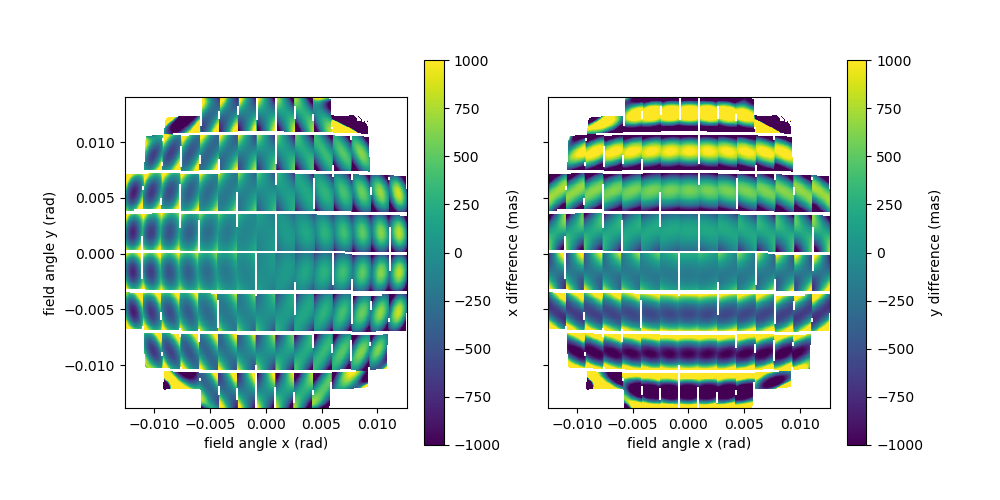
\includegraphics[width=\columnwidth]{figures/CameraOrder6_Order1_comp.png}
\caption{Comparison between the fit 6th-order detector model for the HSC camera and an affine (i.e. first order) model for the transformation between pixels and field angle.}
\label{fig:cam order 1 comp}
\end{figure}
\begin{figure}
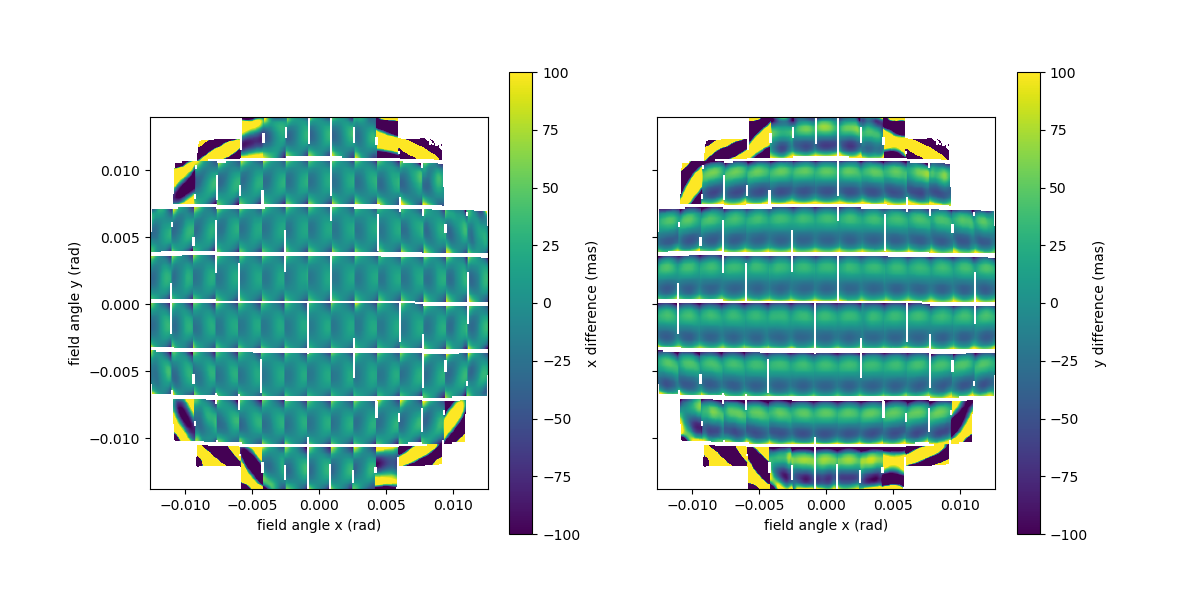
\includegraphics[width=\columnwidth]{figures/CameraOrder6_Order2_comp.png}
\caption{Comparison between the fit  6th-order detector model for the HSC camera and a second-order model for the transformation between pixels and field angle.}
\label{fig:cam order 2 comp}
\end{figure}

\subsection{Apparent motion of objects}\label{sec:Motion}
One of the motivations for moving to the \texttt{gbdes} package was its ability to fit proper motion and parallax. Fitting these motions is currently optional in \texttt{gbdesAstrometrifFitTask}, in order to allow for situations like fitting data that has been simulated without apparent motions, or fitting data with a very short time baseline where allowing apparent motion would add unwanted flexibility. In \texttt{gbdesAstrometricFitTask}, proper motion and parallax fitting are turned on by setting the configuration parameter \texttt{fitProperMotion=True}.
The equations for the position of an object $m$ is then
\begin{equation}
RA_m(t) = RA_{m, t_0} + PM_{RA, m}t + \pi \;P_{RA}(t, RA, Dec)
\end{equation}
\begin{equation}
Dec_m(t) = Dec_{m, t_0} + PM_{Dec, m}t + \pi \;P_{Dec}(t, RA, Dec)
\end{equation}
where $(RA, Dec)_m(t)$ is the observed position of object $m$ at time $t$, $(RA, Dec)_{m, t_{0}}$ is the position at the reference epoch $t_0$, $PM_{RA,Dec} $ is the proper motion of the object, $\pi$ is the parallax of the object, and $P_{RA, Dec}$ is the parallax factor determined by the time $t$ along with the (RA, Dec) of the object.

Figures~\ref{fig:pm gaia comp} to \ref{fig:parallax sigma} show the fits for proper motion and parallax compared to the GAIA DR3 values, along with the uncertainty in the fits as a function of magnitude, when fitting the COSMOS Ultradeep z-band data.
\begin{figure}
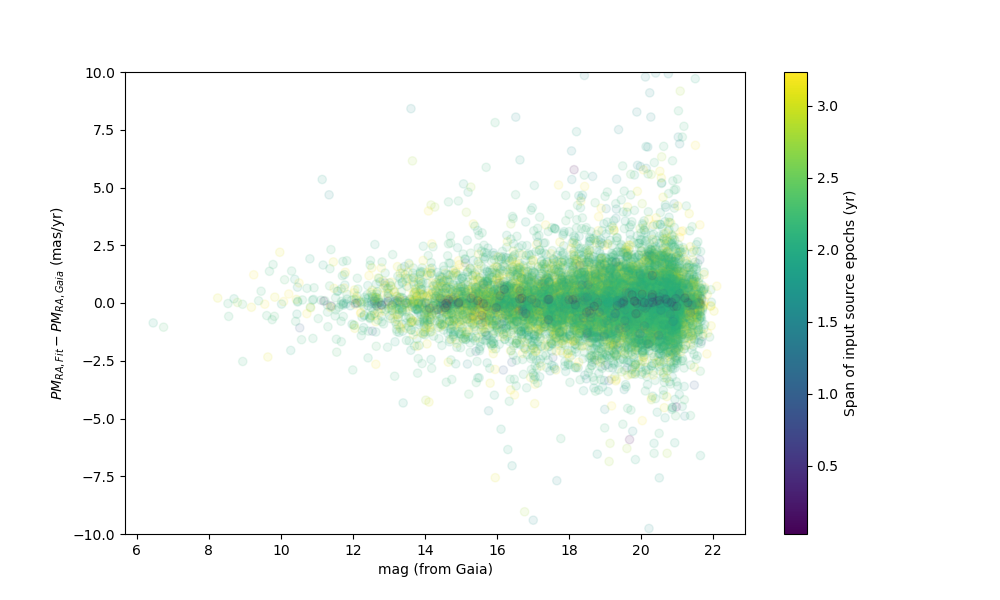
\includegraphics[width=\columnwidth]{figures/pm_ra_gaia_comp_9813.png}
\caption{Comparison between the values fit for the proper motion (in RA) and the values from the GAIA DR3 catalog.}
\label{fig:pm gaia comp}
\end{figure}
\begin{figure}
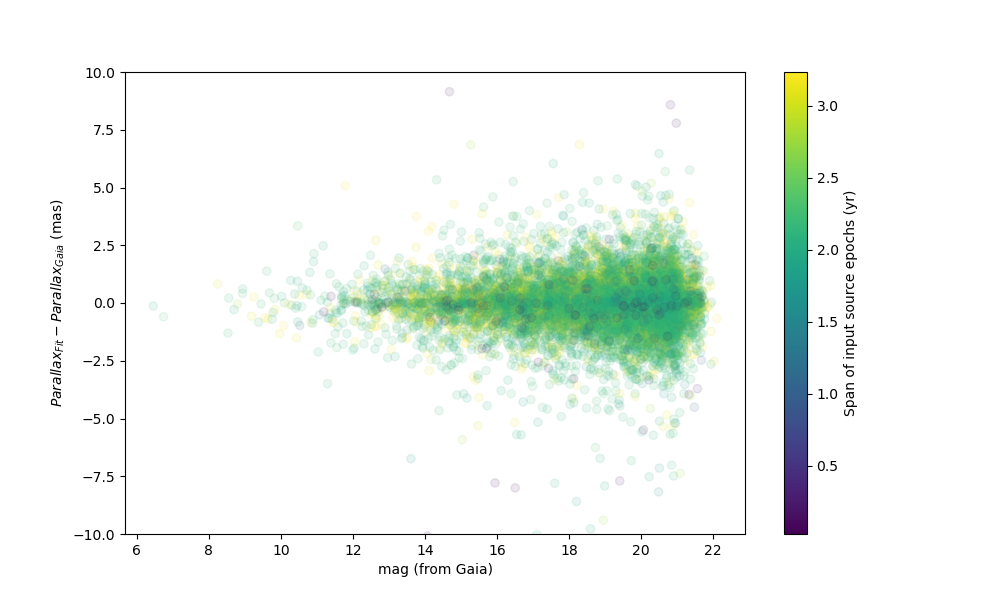
\includegraphics[width=\columnwidth]{figures/parallax_gaia_comp_9813.png}
\caption{Comparison between the values fit for the parallax and the values from the GAIA DR3 catalog.}
\label{fig:parallax gaia comp}
\end{figure}
\begin{figure}
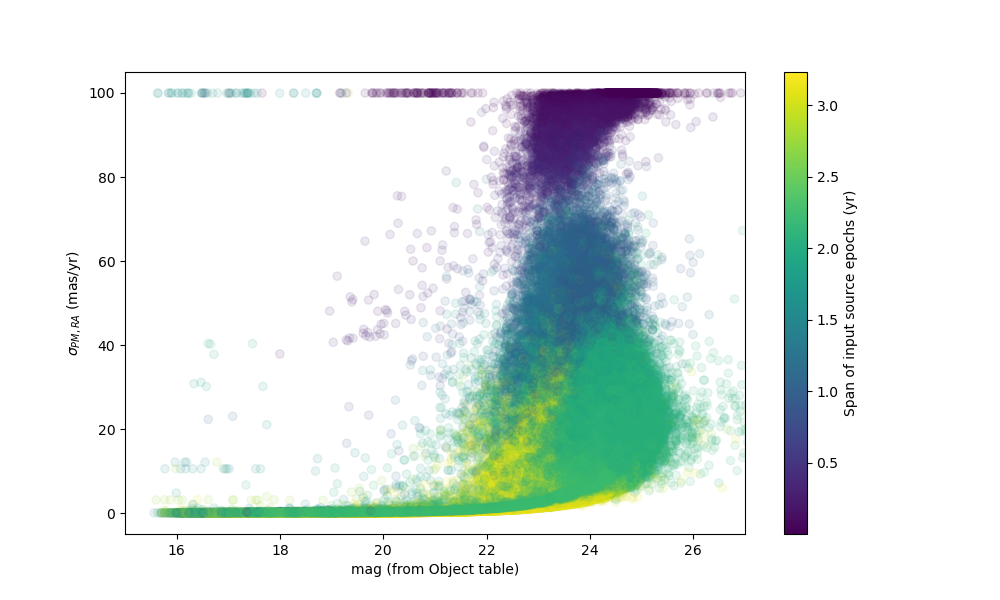
\includegraphics[width=\columnwidth]{figures/pm_ra_sigma_9813.png}
\caption{Uncertainty in the proper motion (in RA) fit as a function of the object magnitude. The color signifies the timespan between the first and last epoch of the input sources for each object.}
\label{fig:pm ra sigma}
\end{figure}
\begin{figure}
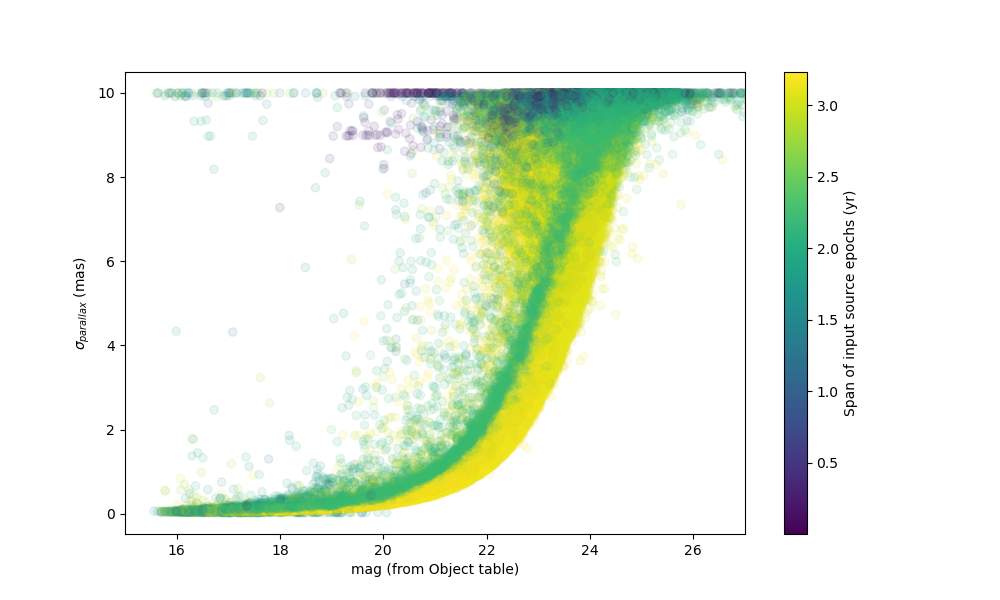
\includegraphics[width=\columnwidth]{figures/parallax_sigma_9813.png}
\caption{Uncertainty in the parallax fit as a function of the object magnitude. The color signifies the timespan between the first and last epoch of the input sources for each object.}
\label{fig:parallax sigma}
\end{figure}


\subsubsection{Differential Chromatic Refraction}\label{sec:dcr}
Another optional correction can be made to the observed position of an object in order to account for Differential Chromatic Refraction (DCR). The Hyper Suprime-Cam data is not affected by this issue because of a color corrector, so this had not been a pressing focus for the development of the astrometric model. However, it is possible with the \texttt{gbdes} package, and has been tested on simulated data for ComCam. Turning on the color correction is done by setting the \texttt{gbdesAstrometricFitTask} configuration variable \texttt{useColor} to be True.

The correction currently implemented for DCR takes the form
\begin{equation}
\Delta \symbf{x_i} = \symbf{D}_{visit} \; c_m
\end{equation}
where $\symbf{D}_{visit}$ is the DCR coefficient determined by the pointing and atmospheric conditions of a given exposure and $c$ is the color parameter for object $m$. 

The main driver in variability of the DCR coefficient is the pointing, so $\symbf{D}_{visit}$ can be modeled generally by the equation
\begin{equation}
\symbf{D}_{visit} = D_{band} \; \mathrm{tan}(z) \symbf{\hat{p}}
\end{equation}
where $z$ is the zenith distance, $\symbf{\hat{p}}$ is the unit sky vector towards zenith, and $D_{band}$ is a constant per-band that is fit to the ensemble of observations. Figure~\ref{fig:dcr} shows the linear relationship between the $D_visit$ fit per visit and the pointing, using simulated ComCam data.
\begin{figure}
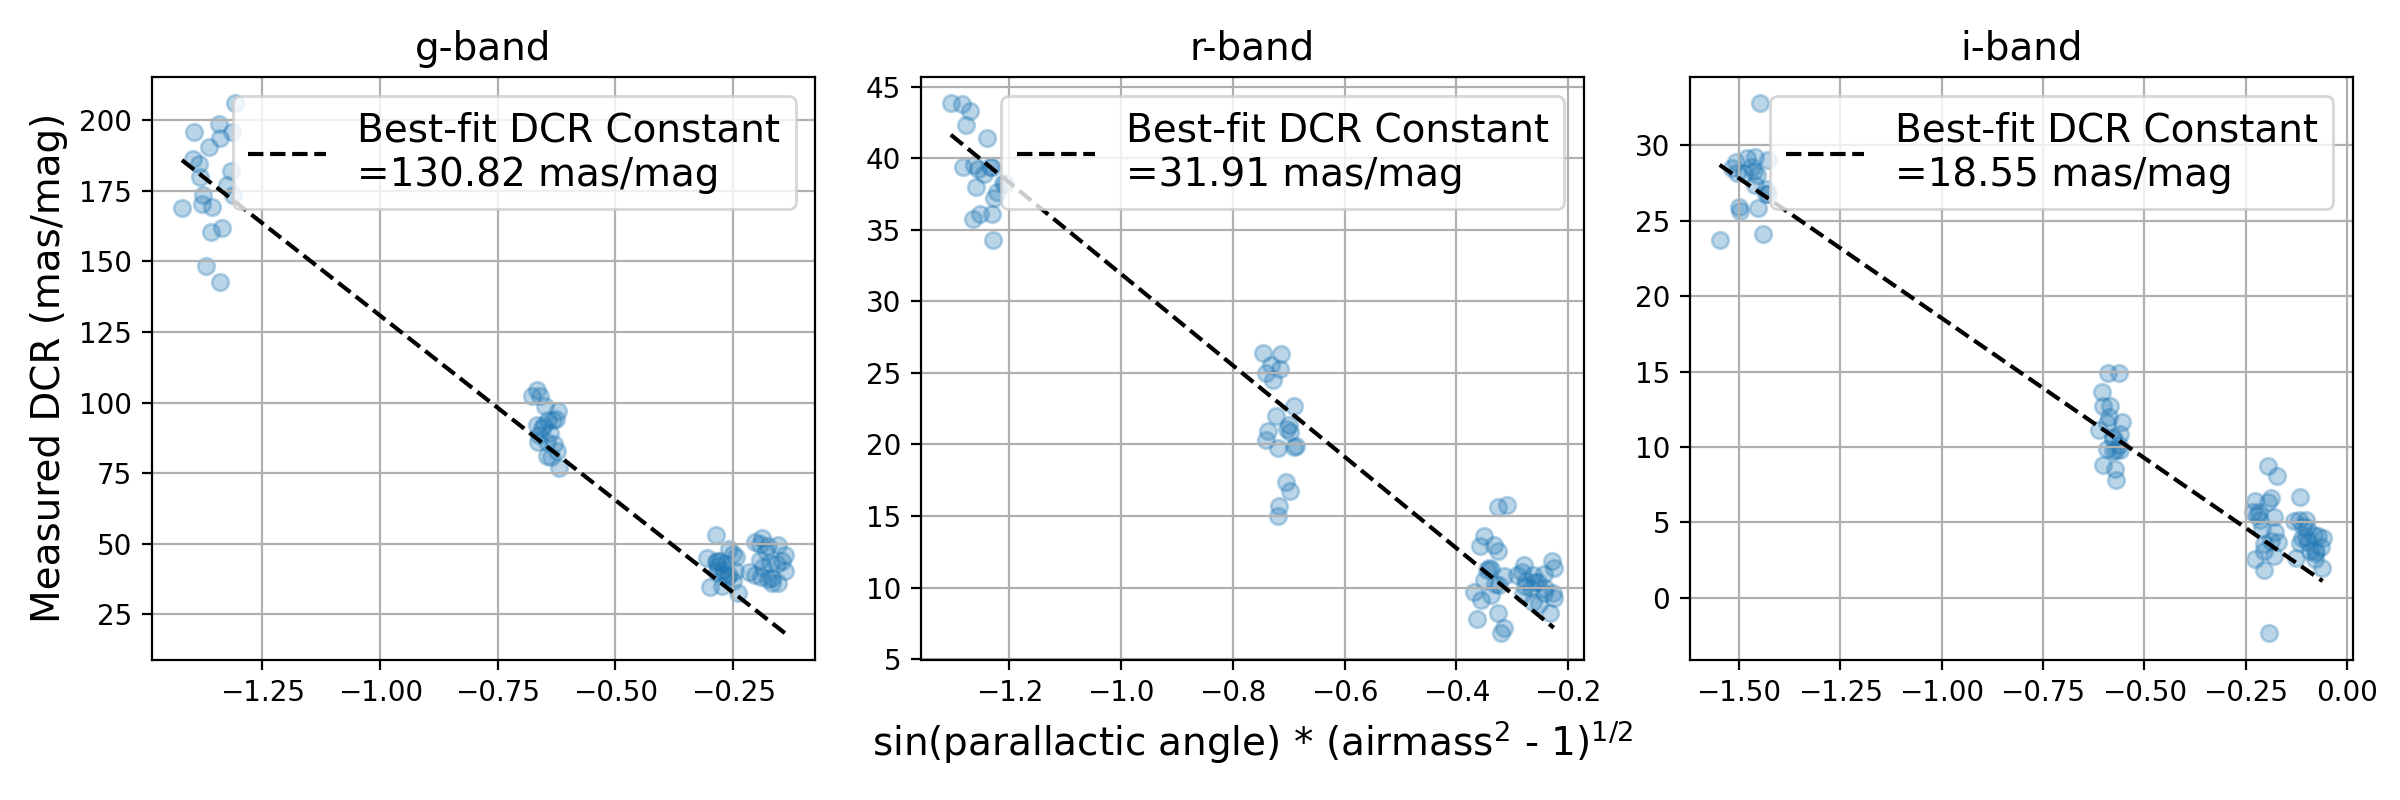
\includegraphics[width=\columnwidth]{figures/dcr_demo.png}
\caption{Fit values for $D_{band}$ as a function of the telescope pointing. }
\label{fig:dcr}
\end{figure}
However, given the large number of sources per visit that are expected from LSST, we can likely get a better fit of the effects of DCR by fitting $D_{visit}$ per exposure in order to allow for time-dependent atmospheric effects.

The default color used is $g - i$, but this is configurable in the task. The magnitudes used to calculate the color come from the \texttt{fgcmCal} calibration of isolated stars, meaning that colors are not available for all objects due to selection differences. %Figure <TODO: figure here> shows the fit residuals as a function of color at a range of airmasses, using simulated ComCam data.



\section{Fitting Modes}\label{sec:modes}
The baseline mode for fitting the astrometric model, as described in Section~\ref{sec:final}, is to fit all of the visits in a given band that are overlapping with a given tract of the sky. However, the model fitting can objectively be improved by using larger amounts of data, and there are scenarios, which will be common for ComCam and in the early days of LSST, where there will not be enough data per tract in a given band. Because of this, a number of different running modes have been developed with an eye towards what will be needed during commissioning.

\subsection{Multiband fitting}
The astrometric model is expected to be different from band to band due to differences in transmission through both the atmosphere and the telescope optics and camera. However, the true positions of the sources are obviously the same regardless of the filter through which they are observed. Fitting multiple band simultaneously thus provides a stronger constraint on this aspect of the model and leads to a fit with greater precision. Running with multiple bands is done by the task \texttt{GbdesAstrometricMultibandFitTask}, which inherits from \texttt{GbdesAstrometricFitTask} and is algorithmically identical. Note that this is independent from the DCR fitting described in Section~\ref{sec:dcr}.

The multiband fit is currently significantly slower than in the single band task, most likely because the matrix that must be inverted in order to perform the fit scales with $N_{band}^2$. However, the matrix in question is block diagonal, so improving the fitter by using this fact should improve the runtime problem, since the fit would then scale as $N_{band}$. Until this is implemented, the multiband running mode is only recommended in cases where there is a very small number of visits per band ($\lesssim10$).

\subsection{"Global" fitting}
\texttt{GbdesGlobalAstrometricFitTask} is another class inheriting from \texttt{GbdesAstrometricFitTask} that adds the option to fit the astrometric model on sets of visits (almost) regardless of their location on the sky, rather than being limited to only visits overlapping with one tract. The advantage of this approach is that the static camera part of the astrometric model can be better constrained with more input visits. The planned use case for this task is not to actually fit the astrometric model for all available visits at the same time, but to allow for fitting the static camera model on a selection of visits from potentially disjoint areas on the sky. By doing this, good-seeing data taken from a number of different fields on the sky (such as the deep-dithered star fields proposed for commissioning) can be used to fit the astrometric model. The static part of this model can then be used as a fixed detector model in subsequent fits of new input data from areas of the sky with potentially limited visits (see Section~\ref{sec:DetMod}).

In practice, for the global task, the input visits are split into separate groups of overlapping visits. The extent of each of these sets of visits then becomes a separate "field", which determines the tangent plane on which the astrometric fit is done. Because of this process, each group of visits must span less than a hemisphere, which is why \texttt{GbdesGlobalAstrometricFit} cannot actually be run globally in the scenario where the input visits actually cover the whole sky.

Because the task is not tract-based, it is possible to include the matched sources from \texttt{isolatedStarAssociationTask} as an input to the task. (See Section~\ref{sec:final} for discussion of how this is not possible in the tract-based class.) Thus, it is not necessary to do source-matching in the task, and the resulting catalog of fit star positions is more consistent with that of other calibration tasks (like \texttt{fgcmCal}) that also use the \texttt{isolated\_star\_sources} as input.

Other than these two aspects of the task, the fit done in \texttt{GbdesGlobalAstrometricFitTask} is otherwise identical to that of \texttt{GbdesAstrometricFitTask}.

 \subsection{Building and Using A Camera Model}\label{sec:DetMod}
With a sufficient number of visits, the astrometric fit should be able to construct an extremely accurate model of the camera distortions from the static detector-based part of the \texttt{gbdes} model. During LSST, we may want to construct a camera model using good-seeing images on deep-dithered star fields. Using the "global" version of the astrometric fitter, these images could be fit together to provide a particularly strong constraint on the camera model. There are (at least) two potential uses for this model:
 
First, it can be used as input when performing the astrometric fit on tracts of the sky where there are a small number of visits. In this case, allowing both the per-detector and per-visit parts of the model to vary will result in overfitting. By using a per-detector model that has been trained on a large amount of data, and then holding that fixed, we can guard against this. In practice, this is done by running the fitter on some training set of visits with the configuration option \texttt{saveCameraModel=True}, then fitting new data with the previous run as an input to the pipeline task and with the configuration option \texttt{useInputCameraModel=True}. Figure~\ref{fig:inputcam} shows the improvement in $\chi^2 / dof$ for validations sources that were withheld from the astrometric fit when using an input camera model compared to letting the model be fit freely.
\begin{figure}
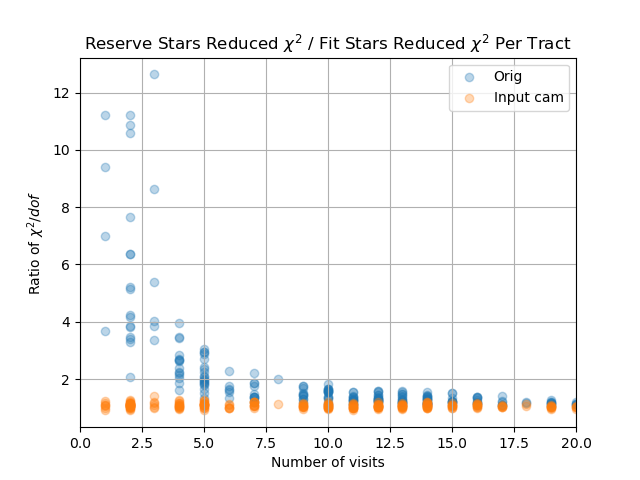
\includegraphics[width=\columnwidth]{figures/inputCamera_demo.png}
\caption{Ratios between the reduced $\chi^2$ between validations sources and fit sources for each tract in z-band from the HSC PDR2 dataset, plotted versus the number of visits going into the fit. Blue points show the ratio when the camera model is free to vary. Orange points show the ratio when using a fixed camera model, fit to a large number of visits. Note that the x-axis is cut off at $20$ visits, since above this point the difference in the two scenarios becomes negligible.}
\label{fig:inputcam}
\end{figure}

Second, the camera model can be fed back into the initial single frame processing in the LSST pipeline. Currently, the initial WCS for images comes from combining the telescope pointing with a model for the camera distortions that is hard-coded in the relevant \texttt{obs\_} package. This model may be theoretically derived or fit from some initial set of observations. This could potentially be improved by using a model generated by the astrometric fitter in the case where the theoretical model does not perfectly capture the real data, or where the camera evolves over time, both very likely scenarios. Again, we can fit the camera model in \texttt{gbdesAstrometricFitTask} using some selected set of high-quality data, potentially from a range of pointings. This is then converted into a \texttt{lsst.afw.cameraGeom.Camera} object and fed into the single frame processing as a pipeline task input, rather than imported from the \texttt{obs\_} package. A further advantage of this approach is that changes in the camera over time can be accounted for by splitting observations into separate stable periods, then using exposures from each period to fit a camera model that can be used for the rest of the exposures from that same period. 

To construct a \texttt{lsst.afw.cameraGeom.Camera} object, \texttt{gbdesAstrometricFitTask} should be run with the configuration option \texttt{saveCameraObject=True}.

\section{Outstanding issues}\label{sec:out}
There are a few known issues that we plan to work on, but which are either in early stages of development or are still in the planning stage:
\begin{itemize}
\item \textbf{Modeling Atmospheric Turbulence} While exposure times for the HSC precursor data are generally around $300$ seconds, the exposure times for LSST will be either $15$ or, more likely, $30$ seconds. Because of this, atmospheric turbulence is expected to have much stronger effects. \cite{Fortino2021} and \cite{Leget2021} showed that it is possible to model astrometric residuals due to atmospheric turbulence using Gaussian Processes. Initial tests showed that a Gaussian Proceses model was able to capture a large portion of the structured astrometric residuals in simulated ComCam data. Figures~\ref{fig:gp vec} through~\ref{fig:gp resid} show the results of the Gaussian Processes fit for a sample exposure.
\begin{figure}
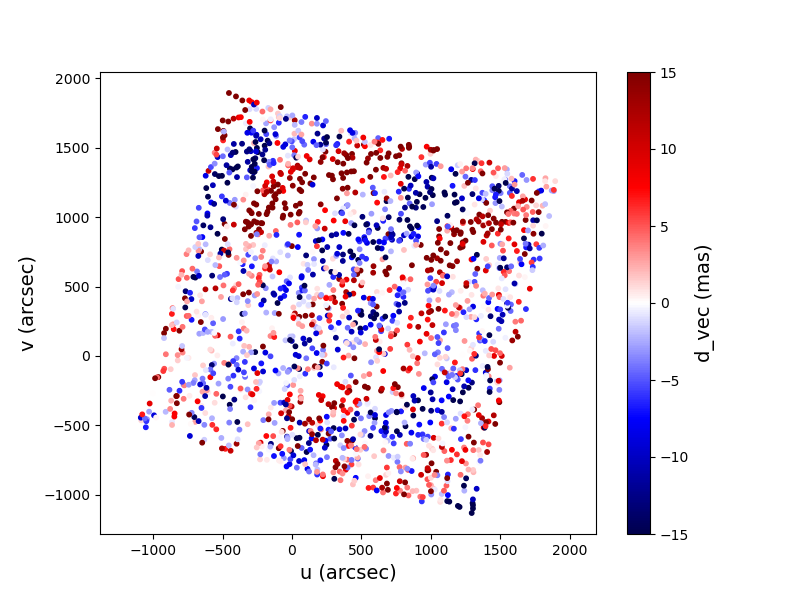
\includegraphics[width=0.7\columnwidth]{figures/vec_test_dv.png}
\caption{Sample astrometric residuals for a simulated ComCam exposure, fit with a low-order polynomial in order to not fit atmospheric turbulence.}
\label{fig:gp vec}
\end{figure}
\begin{figure}
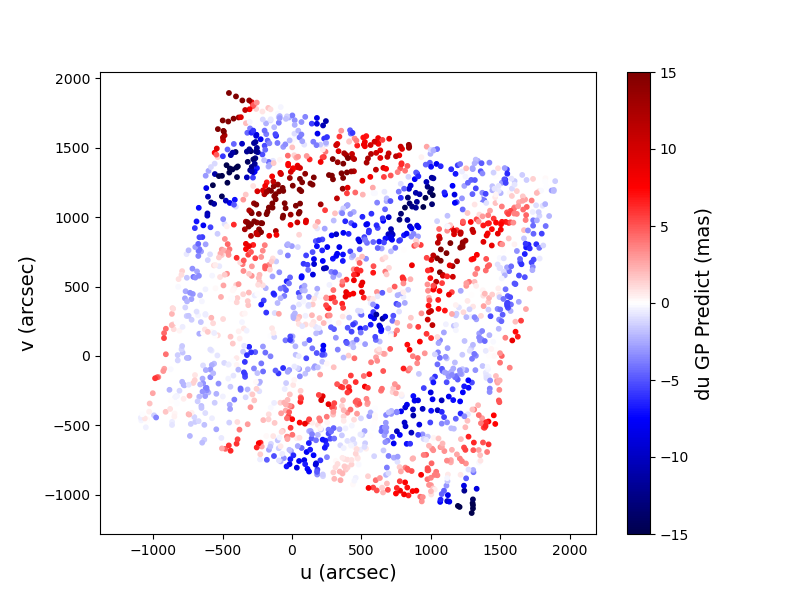
\includegraphics[width=0.7\columnwidth]{figures/predict_test_dv.png}
\caption{Gaussian Processes prediction for the residuals in Figure~\ref{fig:gp vec}.}
\label{fig:gp predict}
\end{figure}
\begin{figure}
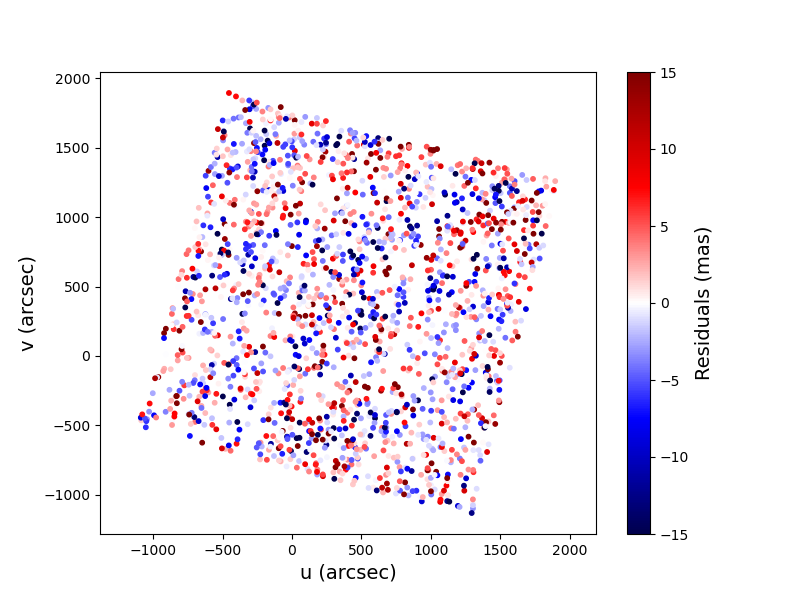
\includegraphics[width=0.7\columnwidth]{figures/resid_test_dv.png}
\caption{Difference between the astrometric residuals and their prediction using Gaussian Processes.}
\label{fig:gp resid}
\end{figure}
However, more work is necessary to add this to the pipeline. We will need to confirm that it works well in a larger range of observing conditions on real data, and to ensure that it is not prohibitively expensive in terms of computing resources.
\item \textbf{Evolution in the Camera} We know that cameras evolve over time, corresponding to various factors such as when the instrument is warmed up and cooled down again. These changes in the instrument lead to changes in the astrometric distortion, which are visible as discontinuities in the distribution of the best-fit visit model parameters. The most straightforward approach to dealing with this will be to run \texttt{gbdesAstrometricFit} separately for each period of relative stability. A more sophisticated approach might be to allow per-epoch camera models that are fit simultaneously, but it is not clear whether the potential improvement in precision will be worth the added complexity in the fit. \item \textbf{Detector Effects} \cite{Bernstein2017} and others have shown that detector electronics and imperfections in the silicon can cause systematic effects in the astrometry, on the scale of a few milliarcseconds for DECam (a similar scale was found for HSC in \citealt{Leget2021}). These effects, which are expected to be static, can be accounted for by adding an additional mapping to the astrometric model. This mapping can be fit by looking at the mean astrometric residuals from a large number (likely at least $1000$) of visits, or can potentially be fit from flats. This mapping would take the form of an additive per-pixel constant vector that would be applied before the per-detector and per-visit maps.
\item \textbf{The Astrometric Solution for Objects other than Calibration Objects} Five-parameter fits for the coordinates, proper motions, and parallaxes for the bright, isolated point sources that are used in the astrometric fit are a necessary byproduct of the astrometric fit. The fits for these sources will be published as \texttt{CalibrationObjects}, possibly with their calibrated fluxes. However, in the long term, we also need to have the same information for the ensemble of objects produced by the pipeline.

In the near to medium-term, we plan to also provide full astrometric fits for all matched sources. This will use the planned, but not yet implemented, table of Object-Source matches, then fit the $5$-parameter solution for these objects, keeping the pixel-to-sky coordinate transforms fixed. This will yield the $5$-parameter astrometry for those objects that are bright enough to be measured in individual visits. However, these fits are expected to be more affected by blending ambiguity than for the isolated \texttt{CalibrationObjects}.

In the longer term, we will provide astrometric fits for all objects, but the method for doing this is still in the planning stages. Potential strategies for doing this include forward-modeling of the per-visit postage-stamps of each object, getting per-visit positions by doing forced centroiding, or measuring centroids in difference-image forced photometry. In some cases, we may want to fit the astrometric solution using object positions in coadded images, stacked either by time period or by season (to isolate parallax). We assume that any of these strategies will require a large number of observations and a time baseline of at least a couple years, which is why this is not considered a priority for development before the survey start.
\end{itemize}


\appendix
% Include all the relevant bib files.
% https://lsst-texmf.lsst.io/lsstdoc.html#bibliographies
\section{References} \label{sec:bib}
\renewcommand{\refname}{} % Suppress default Bibliography section
\bibliography{local,lsst,lsst-dm,refs_ads,refs,books}

% Make sure lsst-texmf/bin/generateAcronyms.py is in your path
\section{Acronyms} \label{sec:acronyms}
\addtocounter{table}{-1}
\begin{longtable}{p{0.145\textwidth}p{0.8\textwidth}}\hline
\textbf{Acronym} & \textbf{Description}  \\\hline

AP & Alert Production \\\hline
ComCam & The commissioning camera is a single-raft, 9-CCD camera that will be installed in LSST during commissioning, before the final camera is ready. \\\hline
DCR & Differential Chromatic Refraction \\\hline
DECam & Dark Energy Camera \\\hline
DM & Data Management \\\hline
DMTN & DM Technical Note \\\hline
DR3 & Data Release 3 \\\hline
DRP & Data Release Production \\\hline
HSC & Hyper Suprime-Cam \\\hline
LPM & LSST Project Management (Document Handle) \\\hline
LSST & Legacy Survey of Space and Time (formerly Large Synoptic Survey Telescope) \\\hline
PDR2 & Public Data Release 2 (HSC) \\\hline
RA & Right Ascension \\\hline
WCS & World Coordinate System \\\hline
\end{longtable}

% If you want glossary uncomment below -- comment out the two lines above
%\printglossaries





\end{document}
